\begin{savequote}[75mm]
We have arranged a civilization in which most crucial elements profoundly depend upon science and technology.
\qauthor{Carl Sagan (1934-1996)}
\end{savequote}

\chapter{Introduction}
\label{Introduction}

\newpage

\section{Research Objectives}

\newthought{The overarching research objective} of this dissertation can be stated as follows: develop an integrated modeling framework, incorporating data depicting local geographic context, that is capable of quantifying the life-cycle energy-water usage efficiency of proposed new infrastructural systems supporting the reuse of treated municipal wastewater for the purpose of artificial groundwater recharge. In order to achieve this goal the following three canonical problems were identified and addressed in sequential order:

    \begin{enumerate}
         
        \item Given multiple independent objectives -- propose a systematic method for selecting sites that are suitable for the development of new artificial groundwater recharge infrastructure.   
        \item Given multiple independent objectives -- propose a systematic method for routing optimal corridors for new water distribution infrastructure linking a designed treated effluent source to a designated recharge destination.
        \item Given a fixed influent flow rate, a set of mean influent pollutant concentrations, a set of maximum effluent pollutant concentrations, and the topological structure of the effluent distribution network -- propose a systematic method for determining the life-cycle energy-water usage efficiency of an integrated wastewater reuse system 
    
    \end{enumerate}
    
The remainder of this Chapter (0) provides an in-depth background discussion of the both the academic and social relevance of the stated research objective. Subsequent Chapters (1-3) are organized with respect to the various independent research activities that were undertaken to address each of the three canonical problems listed above. The final Chapter (4) provides an in depth analysis of a set five case study implementations that were developed to assess the framework's efficacy in satisfying the stated research objective. 

\section{The Energy-Water Nexus}
  
Nearly all modern industrialized societies rely upon energy generation technologies which are derivative of a thermodynamic process known as a heat engine. In a typical heat engine the chemical energy stored within a fuel source such as coal, petroleum, or natural gas, must be first be released as ambient thermal energy through the process of combustion. The heat engine then, by virtue of its design, converts this ambient thermal energy into mechanical energy for the purpose of performing some sort of meaningful work -- i.e. generating electricity.
    
The history of the advancement of the human species is a story which can be cast in terms of the progressive discovery new, higher density chemical energy stores and their enhanced exploitation via the development of new, ever more sophisticated heat engines \cite{Grubler2003,Grubler2010}. Interestingly however, is the fact that nowhere in our history has there ever occurred a single substantial deviation in the choice of the working fluid that actually performs the crucial energy conversion process within a heat engine: water. For all of the advances which have been made in terms of improved fuel processing, boiler and combustion chamber design, etc., so long as our energy economy continues to rely upon carbon based fuels, water will continue to remain stubbornly positioned as a critical component of nearly all major commercial scale energy systems.
    
As interesting aside, although much of the current rhetoric which is used to support a large scale shift towards renewable energy technologies focuses on the benefits of decarbonization; another key benefit of renewable energy technologies, which may be of equal or greater value going on into the future, is the dramatically reduced water intensity relative to that of traditional heat engine based systems. For example, just as photovoltaic electricity generation systems are associated with minimal carbon emissions, so too do they not require substantial inputs of water to facilitate their operation. This is something to watch out for in the future, particularly in the context of long term infrastructure scale planning excises such as the one that shall be introduced as part of this dissertation.
        
Another technological system which can also be viewed as a foundation pillar of modern industrialized societies is the mechanized disposal of human and animal wastes via engineered sewage conveyance and treatment processes \cite{Angelakis2014}. Here again, the advancement of the human species might alternatively be cast in terms of the progressive improvement in the reliability and efficiency of these systems over time. Furthermore, just as the advancement of our energy system appears to be bounded by the physical properties of the water, so too has the advancement of wastewater management been similarly constrained. 
        
For example, in terms of water treatment processes, the upper bound on process efficiency is determined by \textit{The Second Law of Thermodynamics}. This law states that, for any closed system, there is a tendency for the entropy of that system to increase over time \cite{Jaynes1996}. \textit{Ceteris paribus}, wastewater, a heterogeneous mixture, possesses higher entropy than pure water does. This means that any attempt to purify a polluted wastewater stream must necessarily incur the cost of some energy input to facilitate the requisite reduction in entropy. 
    
In terms of water distribution processes, the key physical determinant of energy efficiency stems from the density of water. At 1000 $kg/m^3$, considerable energy must be expended whenever large quantities of water must be moved over a distance or lifted against an elevation gradient. Many treatment processes utilize pressurized sieving techniques where water is physically pushed through a porous membrane in order to forcibly remove dissolved pollutant species. As a consequence of this practice, the energy inputs required to overcome the previously mentioned entropic gradient are often supplied for the immediate purpose of moving quantities of water from place to place.
    
     \begin{figure}[!h]
       \centering
       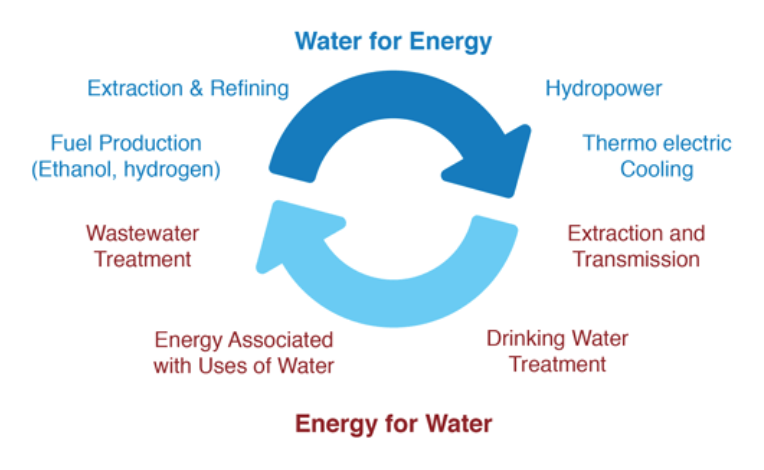
\includegraphics[width=4.5in]{figures/energy-water-nexus-perspectives.png}
       \caption[Perspectives on the Energy-Water Nexus]{Perspectives on the Energy-Water Nexus \cite{Pate2007}}
       \label{fig:energy-water-perspectives}
     \end{figure}
     
The energy-water nexus is a term which has emerged from within the academic research community to describe these types of dynamic interrelationships which are inherent to our energy and water systems. There are two perspectives from which the energy-water nexus can be alternatively studied. The first emphasizes the \textit{water for energy} dimension, and is generally concerned with the study of processes and technologies that are involved with the direct withdrawal and consumption of water for the production of both primary and final energy resources. The second of these perspectives, focuses alternatively on the \textit{energy for water} dimension; investigating processes and technologies which consume energy for the purpose of transmitting or purifying freshwater resources. 
    
     \begin{figure}[!h]
       \centering
       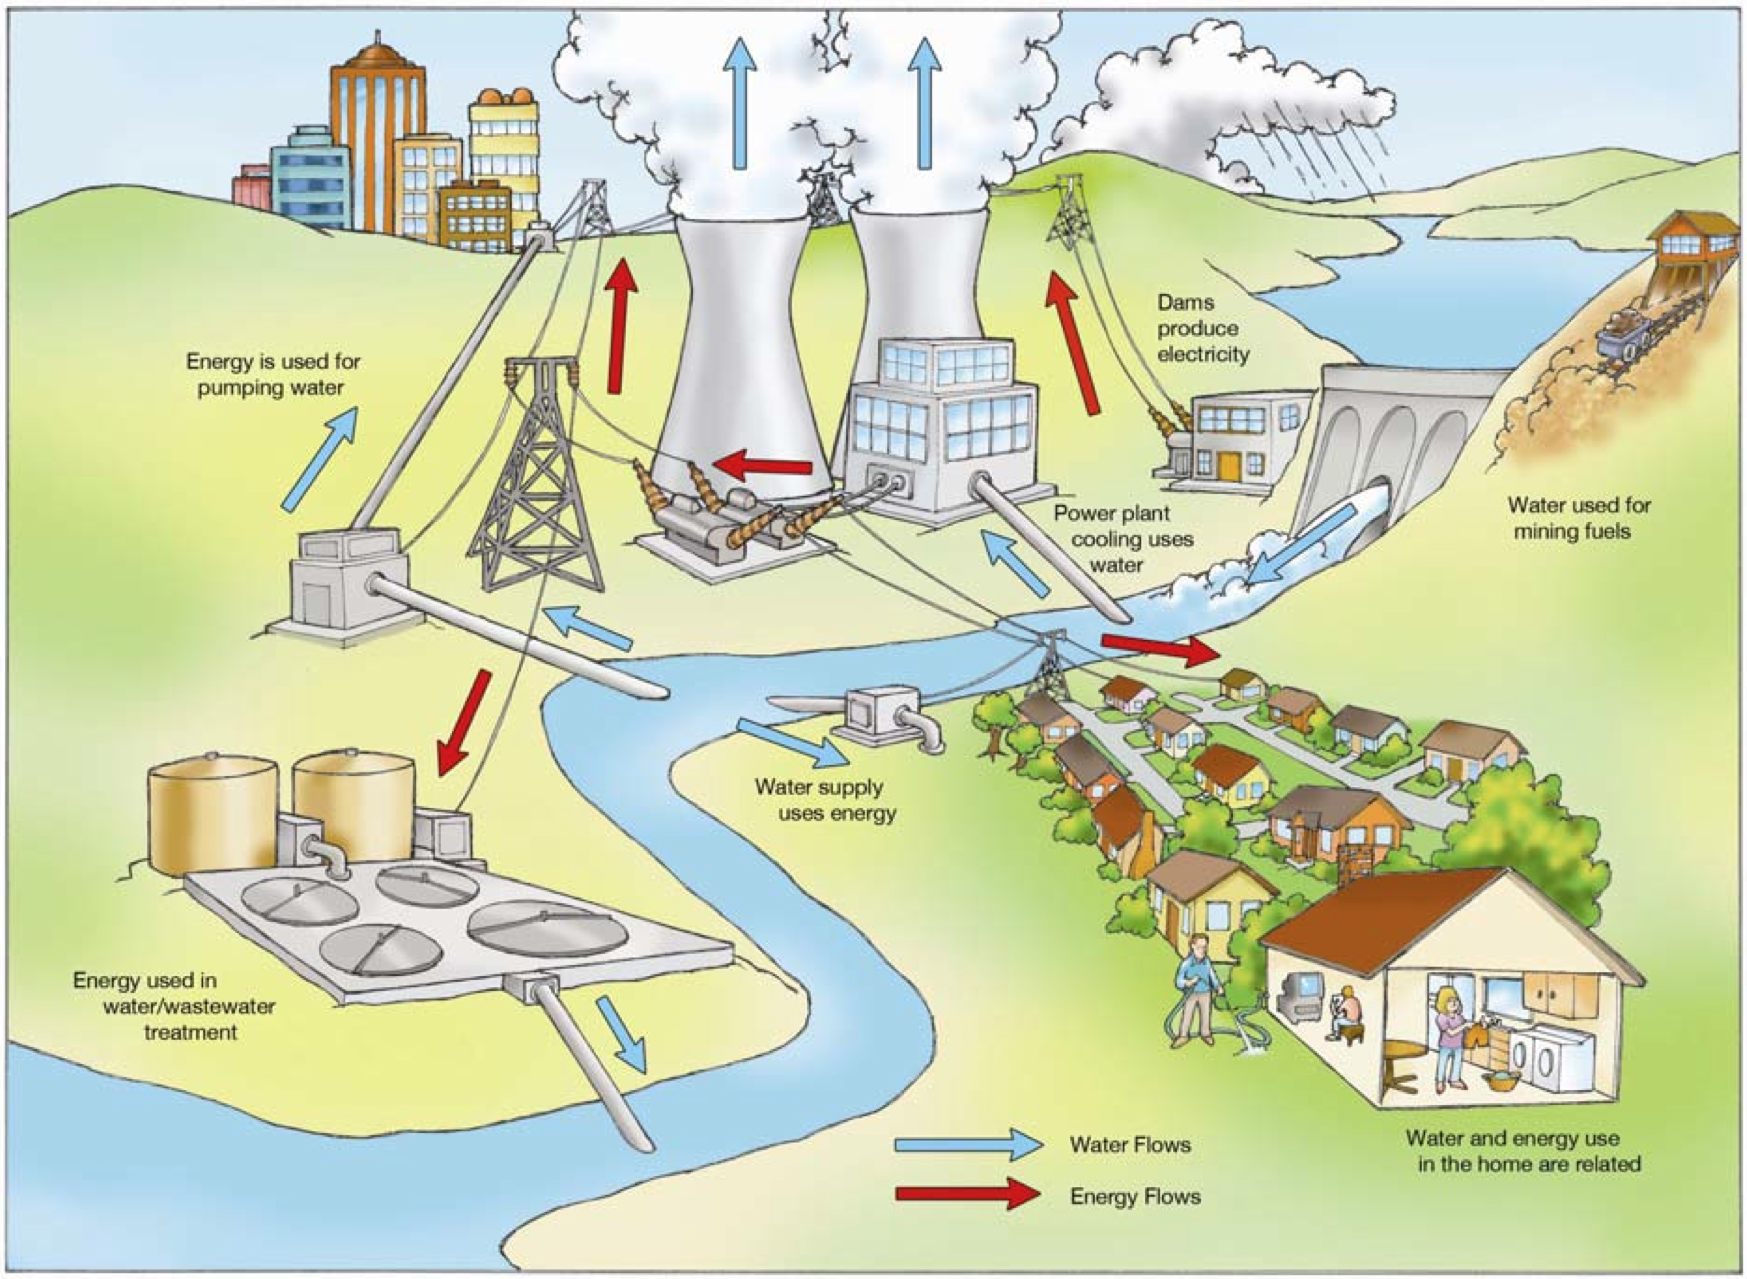
\includegraphics[width=5.5in]{figures/energy-water-nexus-dimensions.png}
       \caption[Dimensions of the Energy-Water Nexus]{The dimensions of the energy-water nexus \cite{Pate2007}}
       \label{fig:energy-water-dimensions}
     \end{figure}
    
Here in the United States, approximately 50\% of total annual freshwater withdrawals are used for the cooling of thermoelectric power plants. Alternatively, roughly 4\% of the nation's total energy consumption is dedicated to the transmission and purification of water and wastewater. While these national figures speak to the overall significance of this issue, the situation becomes more acute when one begins to consider different regional contexts. 
    
The criticality of the energy-water nexus becomes greatly exacerbated in those areas where either water is scarce, energy is scarce, or both. Unfortunately, the state of California suffers from both of these conditions to varying degrees, making the energy-water nexus a frequent source of regional interest within both the academic research and socio-political circles. For example, in a 2005 report published by the California Energy Commission (CEC) it was found that 19\% of the electricity and 32\% of the natural gas consumed within the entire state were used for purpose directly related to the supply and treatment of freshwater resources \cite{Horvath2005}.
    
\section{Water Distribution Systems}
    
One of the main drivers for of this tremendous energy consumption within the state of California is the large scale transfer of freshwater resources between physically distinct hydrologic basins. California is crossed latitudinally by a massive network of interconnected hydraulic engineering projects including pipelines, aqueducts, reservoirs, and pump stations \cite{Schwarzenegger2005, Schwarzenegger2005}. These systems, which have been funded by a mixture of Federal, State, and Local agencies, were designed to reconcile discontinuities between the spatial and temporal distributions of the supply and demand for freshwater resources within the state \cite{Freeman2008}.

       \begin{figure}[!h]
       \centering
       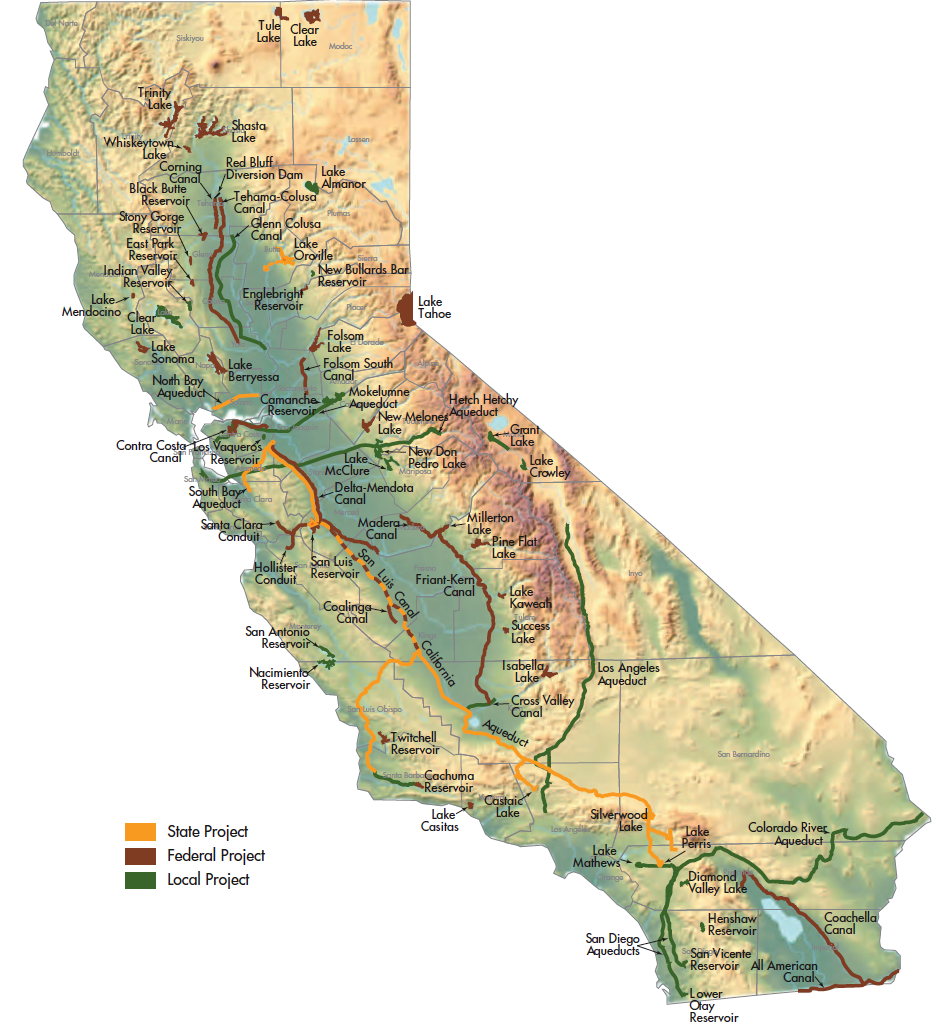
\includegraphics[width=5.5in]{figures/infrastructure.png}
       \caption[Characteristics of Water Distribution Infrastructure]{The geographic extent of water distribution infrastructure in the state of California \cite{Schwarzenegger2005}}
       \label{fig:california-distribution}
     \end{figure}
    
Inter-basin transfers typically involve the movement of water against a considerable elevation gradient. Due to water's previously mentioned high density, there are substantial energetic costs associated with operating the infrastructure required to facilitate these transfers. For example, the bar graph to the right of Figure \ref{fig:infrastructure-energy-intensity} compares the energy intensity of several different sources of municipal water within the state of California \cite{Wilkinson2007}. According to this research water resources which are supplied via inter-basin transfer, either through branches of the State Water Project or through the Colorado River Aqueduct, rank very poorly in terms of energy usage efficiency relative to a number of other water supply systems.

     \begin{figure}[!h]
       \centering
       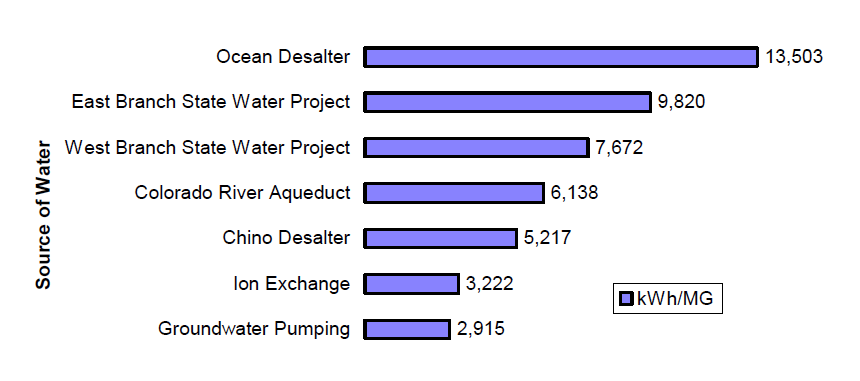
\includegraphics[width=5.5in]{figures/energy-intensity.png}
       \caption[Energy Intensity of Water Distribution Infrastructure]{The geographic extent of water distribution infrastructure in the state California \cite{Klein2005}}
       \label{fig:infrastructure-energy-intensity}
     \end{figure}
     
\section{Wastewater Treatment}

The term \textit{wastewater treatment} refers to a set of physical and chemical processes that have been individually designed and are collectively composed for the purpose of removing a suite of physical, chemical, and/or biological contaminants from a quantity of water \cite{Metcalf1991}. The operational goal of a wastewater treatment process is typically defined in terms of a set of desired effluent pollutant concentrations that are sufficiently low to enable that effluent to be used for a specific end-use application \cite{Asano2007}. Crucially implicit in this definition therefore, is the notion that the precise combination and configuration of the individual, atomic treatment processes, will vary on the basis of the purity requirements associated with the anticipated end-use application. Figure \ref{fig:process-flow-diagram} provides a high level view of the separate treatment processes that are typical to modern wastewater treatment facilities; assigning them to a somewhat informal hierarchy consisting of: primary treatment, secondary treatment, and tertiary treatment \cite{Asano2007}.

    \begin{figure}[!h]
       \centering
       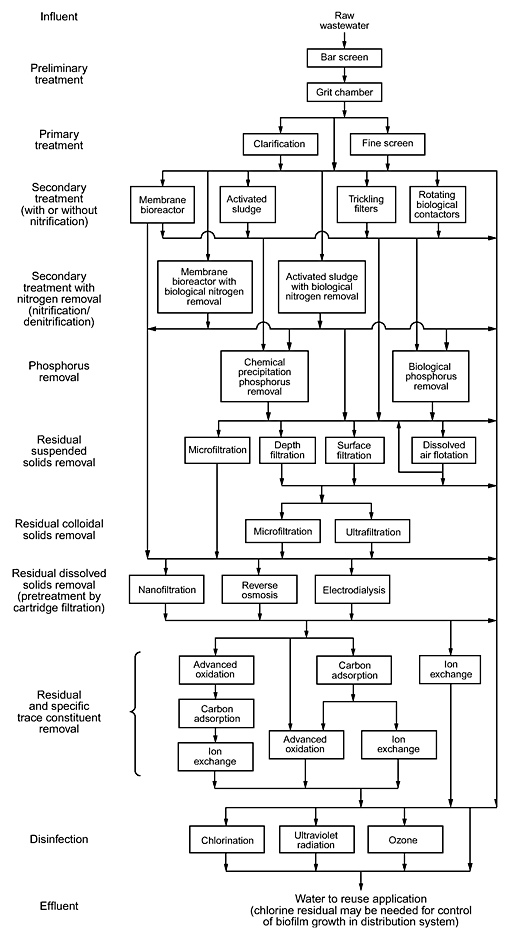
\includegraphics[width=4in]{figures/process-flow.png}
       \caption[Process Flow Diagram of Wastewater Treatment Methods]{Process flow diagram of various wastewater treatment methods \cite{Asano2007}}
       \label{fig:process-flow-diagram}
     \end{figure}

The collection of processes described in Figure \ref{fig:process-flow-diagram} represent the required suite of treatment operations necessary to produce effluent water that is suitable for groundwater recharge applications (also known as: indirect potable reuse) given a normal stream of influent municipal wastewater. Typically, wastewater treatment plants (WWTPs) -- normal in the sense that they are producing treated effluent from generic municipal sources for release into natural surrounding environs -- are only required to provide up to a secondary treatment level \cite{Asano2007}. This level of treatment, on the diagram provided in Figure \ref{fig:process-flow-diagram}, corresponds to the fourth row of processes from the top. As the figure shows, providing treated effluent for reuse applications necessitates the implementation of as many a seven additional layers of tertiary treatment in order to manage issues such as suspended colloids, disinfection, and phosphorous removal \cite{Tchobanoglous2003}.

This hierarchy of treatment processes depicted in Figure \ref{fig:process-flow-diagram} is only meant to be representative of the types of processes that are typically required for reuse applications. In reality however, neither the rigid segregation of treatment processes nor the association of each treatment level with a set of designated end-uses have been precisely codified into a coherent regulatory framework at the Federal level. In general, primary and secondary treatment are Federally mandated as part of the generic WWTP under provisions of the Clean Water Act \cite{NRC2008,CDHS2001}. However, tertiary treatment processes and requirements for their application in the context of different desired end-use applications, are, at present, regulated at the state or local levels in a more ad-hoc manner. Figure \ref{fig:use-categories} attempts to illustrate the complexity of this landscape by mapping treatment levels to different end-use types, with annotations where additional restrictions may apply \cite{NRC2008,Romero-Hernandez2004}.

     \begin{figure}[!h]
       \centering
       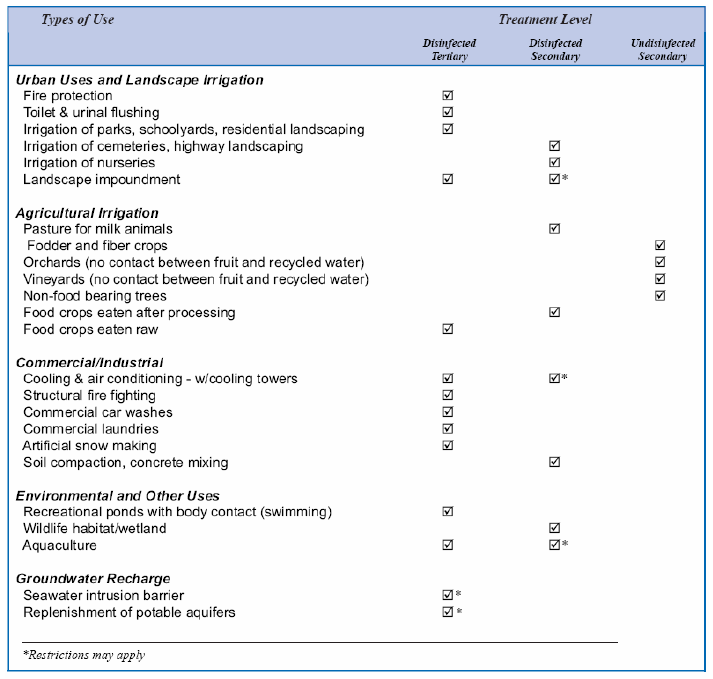
\includegraphics[width=5.5in]{figures/use-categories.png}
       \caption[Appropriate End Use Categories for Different Levels of Treated Wastewater]{Appropriate End Use Categories for Different Levels of Treated Wastewater \cite{Klein2005}}
       \label{fig:use-categories}
     \end{figure}
     
\section{Wastewater Recycling and Reuse}
    
Over the past ten years the reuse of treated wastewater has emerged as the fastest growing source of new water supply for municipal water districts in the Western United States \cite{Dolnicar2006a,USEPA2012}. There are a variety of reasons for this growth trend. For example, some districts enjoy the degree of self determinism that ownership of a reuse system affords them; particularly in cases where they are beholden to a the whims of a third party water wholesalers or are junior water right holders within their basin. In general however, the primary driving force behind the increased interest in reuse has been down to the fact that treated municipal wastewater is perceived to be an efficient means of new water supply for a number of low quality end use cases \cite{Kennedy2005,CDWR2003}.

If one looks at existing reuse systems, these assumptions regarding system efficiencies appear to be valid. This is because the vast majority of reuse systems which have been implemented to date have taken advantage of favorable circumstances such as where the destination location for the treated effluent is positioned in fairly close proximity to the WWTP. An illustrative example of such a situation might be the use of wastewater which had been subjected to basic secondary treatment for the irrigation of a nearby cemetery or golf course. These types of reuse systems can be thought of as low hanging fruit because the only additional energy process based energy expenditures associated with their operation come from whatever tertiary treatment processes must be added into the WWTP operations to meet the effluent purity requirements associated with the designated end-use. 

More recently however, many municipalities have begun to actively investigate the possibility of expanding both the scale and extent of their reuse operations: capturing larger fractions of their WWTP plants' throughput and distributing the treated effluent to a more diverse portfolio of end-use recipients. Among these proposed new end-use applications, perhaps the most attractive has been for artificial groundwater recharge. 

An artificial groundwater recharge operation is one which takes some stream of input water, it need to necessarily be treated wastewater, and either passively or forcefully introduces it to the subsurface aquifer \cite{Bouwer1999}. The goal of this process is typically undertaken to remedy a condition of overdraft wherein the aquifer has been subjected to increased rates of withdrawals, decreases rates of natural infiltration, or both \cite{Seiler2007}. Typically artificial groundwater recharge systems adopt one of two approaches in terms of the mechanism by which they physically deliver the water back to the subsurface. The first approach is passive -- involving the construction of one or more large scale infiltration basins into which water is pumped and then allowed to percolate into the subsurface through a porous media under the force of gravity \cite{NRC2012}. The second approach is active -- involving the construction of one or more pump wells through which water is forced into the subsurface under the action of a mechanized pump \cite{NRC2012}. 

Due to the considerable cost associated with pump operation as well as the limited recharge capacity associated with each individual wellhead, recharge basins have, up until this point, proven to be far and away the more attractive of the two options in terms of existing facilities. The primary exemption to this rule being locations where the reason that the recharge operations have been undertaken is create a target increase in subsurface hydrostatic pressure for the purpose of mitigating the encroachment of brackish water into the aquifer -- which can often occur in coastal regions -- or for the purpose of halting or redirecting the movement of some subsurface groundwater pollutant plume \cite{Rodrigo2012}. 

Despite the fact that artificial recharge basins take advantage of the force of gravity to introduce the water back into the subsurface they can still be expected to be associated with fairly large operational energy requirements. This is because, for a host of practical engineering as well as political and economic constraints, recharge basins tend not to be constructed as close to the source of their supply water as one might initially think. As a result, considerable amounts of energy must be continually invested to pump water, often against an elevation gradient, from its source of production to the recharge basin where it will ultimately be consumed for the purpose of artificial groundwater recharge. 
              
\section{The Energy-Water Feedback Loop}
 
The suggestion that all forms of artificial groundwater recharge are likely to be associated with non-trivial process based energy demands leads to an interesting question regarding the net life-cycle energy utilization efficiency of reuse systems. This question stems from an understanding of the water usage intensity of various electricity generation technologies can vary significantly and is often much high than one mights initially expect. 
 
For example, Figure \ref{fig:water-consumption-intensity} plots the water usage intensity -- measured in terms of units of water consumed per unit of electric power produced -- for a suite of electricity generation technologies that make up a substantial portion of the municipal energy generation portfolio here in the United States \cite{Averyt2013}. As Figure \ref{fig:water-consumption-intensity} illustrates, depending upon the details of how electricity is produced in a given region, artificial groundwater recharge operations that utilize heavily treated municipal wastewater as their source feedstock have the potential to be associated with significant process energy related water consumption levels at the point of electricity production.
 
       \begin{figure}[!h]
           \centering
           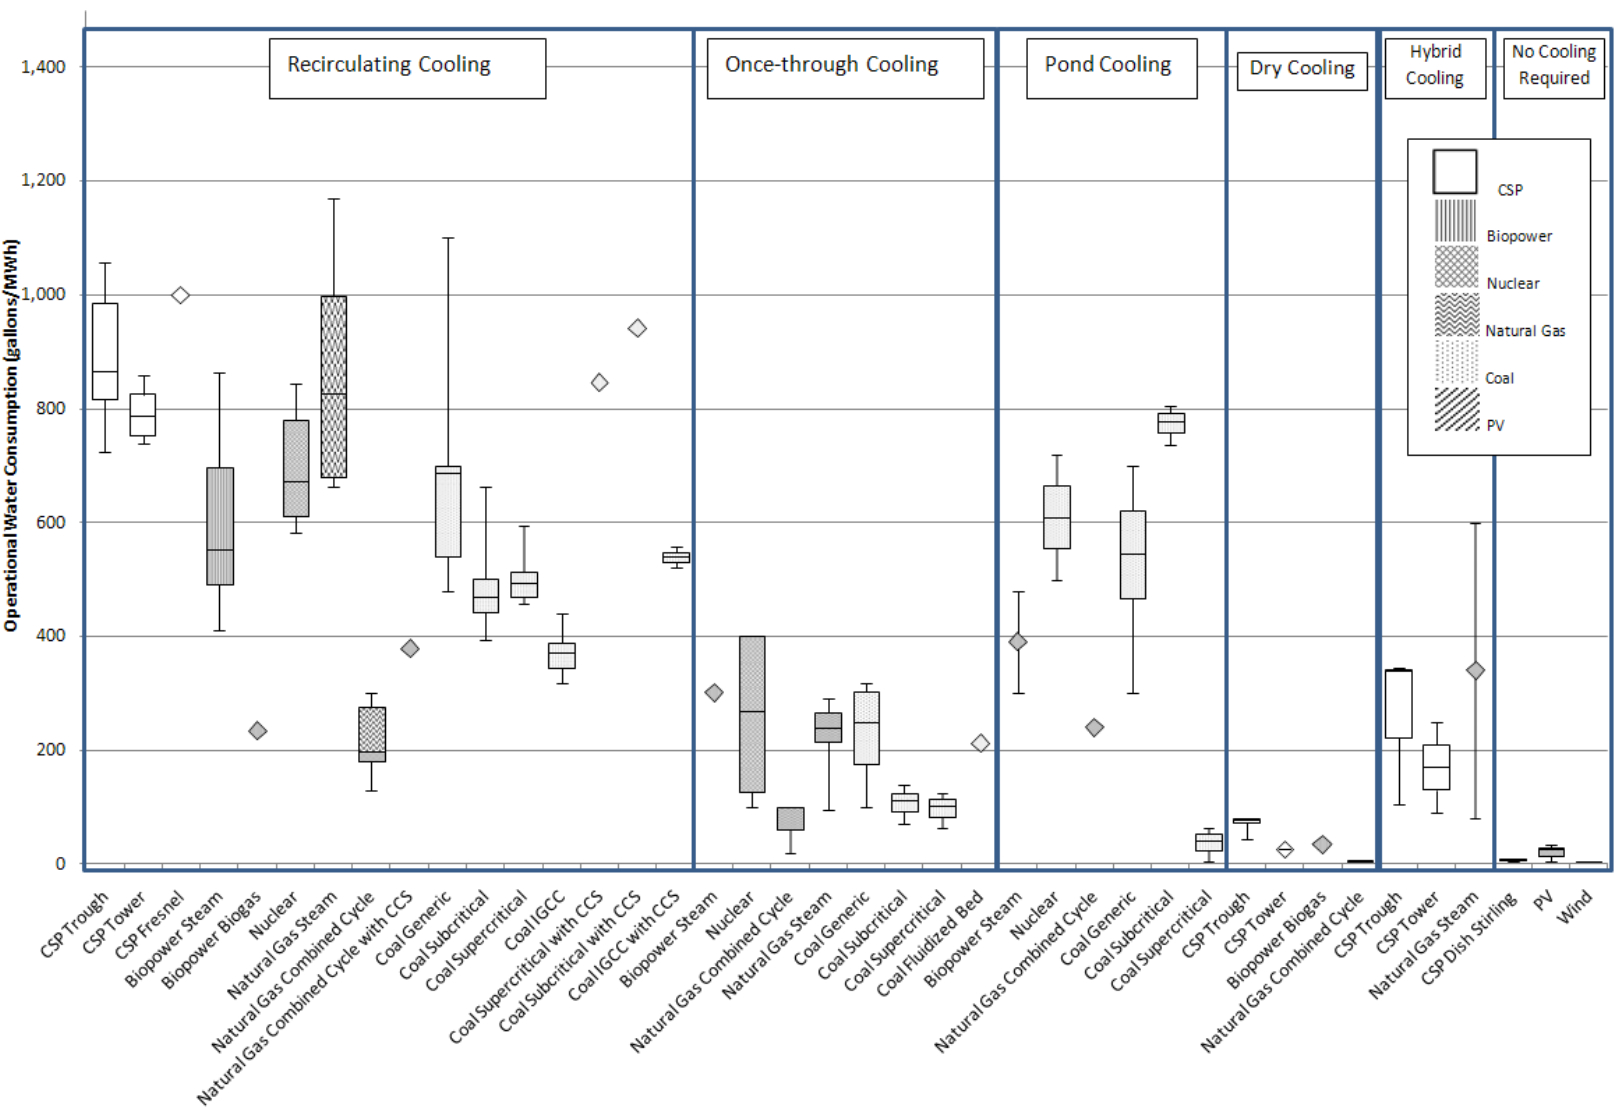
\includegraphics[width=5.5in]{figures/water_consumption_for_energy.png}
           \caption[Water Intensity of Energy Production]{The water consumption intensity, measured in terms of water consumed per unit of electric power produced, for various electricity generation technologies \cite{Averyt2013}}
           \label{fig:water-consumption-intensity}
       \end{figure}
        
In light of the presence of this significant feedback loop, the hypothesis that this dissertation has been designed to test is whether or not there exists a specific set of circumstances in which it may be possible for municipal wastewater reuse systems involving a substantial artificial groundwater recharge components to produce a situation where they are saving some water locally, but at the cost of consuming more water regionally. This hypothesized negative net water savings, at the regional scale, would therefore be the result of water consumption which is embedded in the energy that must be imported to facilitate the reuse and recharge operations.

\clearpage